\documentclass[10pt]{scrartcl}
\usepackage{amsmath,amsthm,amssymb,mathtools,xfrac}
\usepackage{enumerate}
\usepackage[utf8]{inputenc}
%\usepackage{german}
\usepackage{a4wide}
\usepackage{graphics}
\usepackage{graphicx}
\usepackage[T1]{fontenc}
\usepackage{epsfig}
\usepackage{libertine}
\usepackage[pdftex]{hyperref}
\usepackage{refcount}
\usepackage{framed}
\usepackage{xcolor}
\usepackage{multicol}
\usepackage{enumitem}
\usepackage{caption}
\usepackage{gensymb}
\usepackage[export]{adjustbox}

\DeclareMathOperator{\sinc}{sinc}

\topmargin-.5in \textheight9in \oddsidemargin0in \textwidth6.5in

\begin{document}


\begin{minipage}{.5\textwidth}
{\scshape Department of Mathematics and Informatics \\
University of Cologne\\}
\small Prof. Dr. Gregor Gassner \\
\end{minipage}
\begin{minipage}{.3\textwidth}
{\scshape Department of Mathematics \\
Link\"{o}ping University\\}
\small Andrew R. Winters \\
\end{minipage}
\hfill
\begin{minipage}{.15\textwidth}
\begin{flushright}
%\includegraphics[width=3cm]{figs/logo-uni-koeln.jpg}\\
\today
\end{flushright}
\end{minipage}

\begin{center}
{\Large\bfseries
An Introduction to Climate Modeling}\\
\vspace{0.2cm}
{\bfseries Milestone 1 - Geography and Visualization}
\end{center}

\section{Read-in and Plot Geography}

In this milestone, the goal is to read-in the geography information of planet Earth and plot it as a two-dimensional world map.
We consider an equirectangular grid of the Earth, i.e., an equidistant rectangular grid in spherical coordinates, where the grid point $(i, j)$ has the spherical coordinates $(\theta_i, \varphi_j)$, where $\theta_i$ is the latitude between $-90\degree$ south and $90\degree$ north (including the poles) and $\varphi_j$ the longitude between $-180\degree$ west and $180\degree$ east.
The basis for this is the input file
\small\texttt{\detokenize{The_World65x128.dat}}\normalsize, which describes the distribution of the different Earth surface types.
This file contains a matrix $G \in \mathbb{N}^{65 \times 128}$ with entries $g_{ij} \in \{1,2,3,5\}$, where the entry $g_{ij}$ stores the Earth surface type at grid point $(i, j)$.
Here, $1$ represents the Earth surface type \textit{land}, $2$ represents \textit{sea ice}, $3$ represents \textit{snow}, and $5$ represents \textit{ocean}. The grid resolution in longitude and latitude direction is $2.8125^{\circ}$.
The basis for this distribution and grid is from Zhuang et al.\footnote{K. Zhuang, G.R. North, M.J. Stevens, {\em A NetCDF version of the two-dimensional energy balance model based on the full multigrid algorithm}, SoftwareX, Vol. 6, pp. 198-202, July 7, 2017.}
You can proceed as follows:

\begin{enumerate}
\item Write a function \small\texttt{\detokenize{read_geography}}\normalsize, which reads the file \small\texttt{\detokenize{The_World65x128.dat}} \normalsize from the folder \small\texttt{\detokenize{input}} \normalsize and outputs a matrix $T \in \mathbb{N}^{65 \times 128}$  with the classification of the earth surface types.

\item Write a function \small\texttt{\detokenize{robinson_projection}}\normalsize, which maps an equirectangular grid in spherical coordinates to the plane.
For simplicity use the approximate formula by Beineke for the Robinson projection,
\begin{align*}
	&x\left(\theta, \varphi \right) = \frac{\varphi}{\pi}\left(0.0379\hspace{0.05cm}\theta^6 - 0.15\hspace{0.05cm}\theta^4 - 0.367\hspace{0.05cm}\theta^2 + 2.666 \right),\\
	&y\left( \theta, \varphi \right) = 0.96047\hspace{0.05cm}\theta - 0.00857\hspace{0.05cm}\text{sign}\left(\theta\right)\left|\theta\right|^{6.41},
\end{align*}
where $\varphi$ is the longitude and $\theta$ the latitude in radians.
This function should return two matrices $X = x_{ij}$ and $Y = y_{ij}$, where $x_{ij} = x(\theta_i, \varphi_j), y_{ij} = y(\theta_i, \varphi_j)$.

\begin{figure}[h]
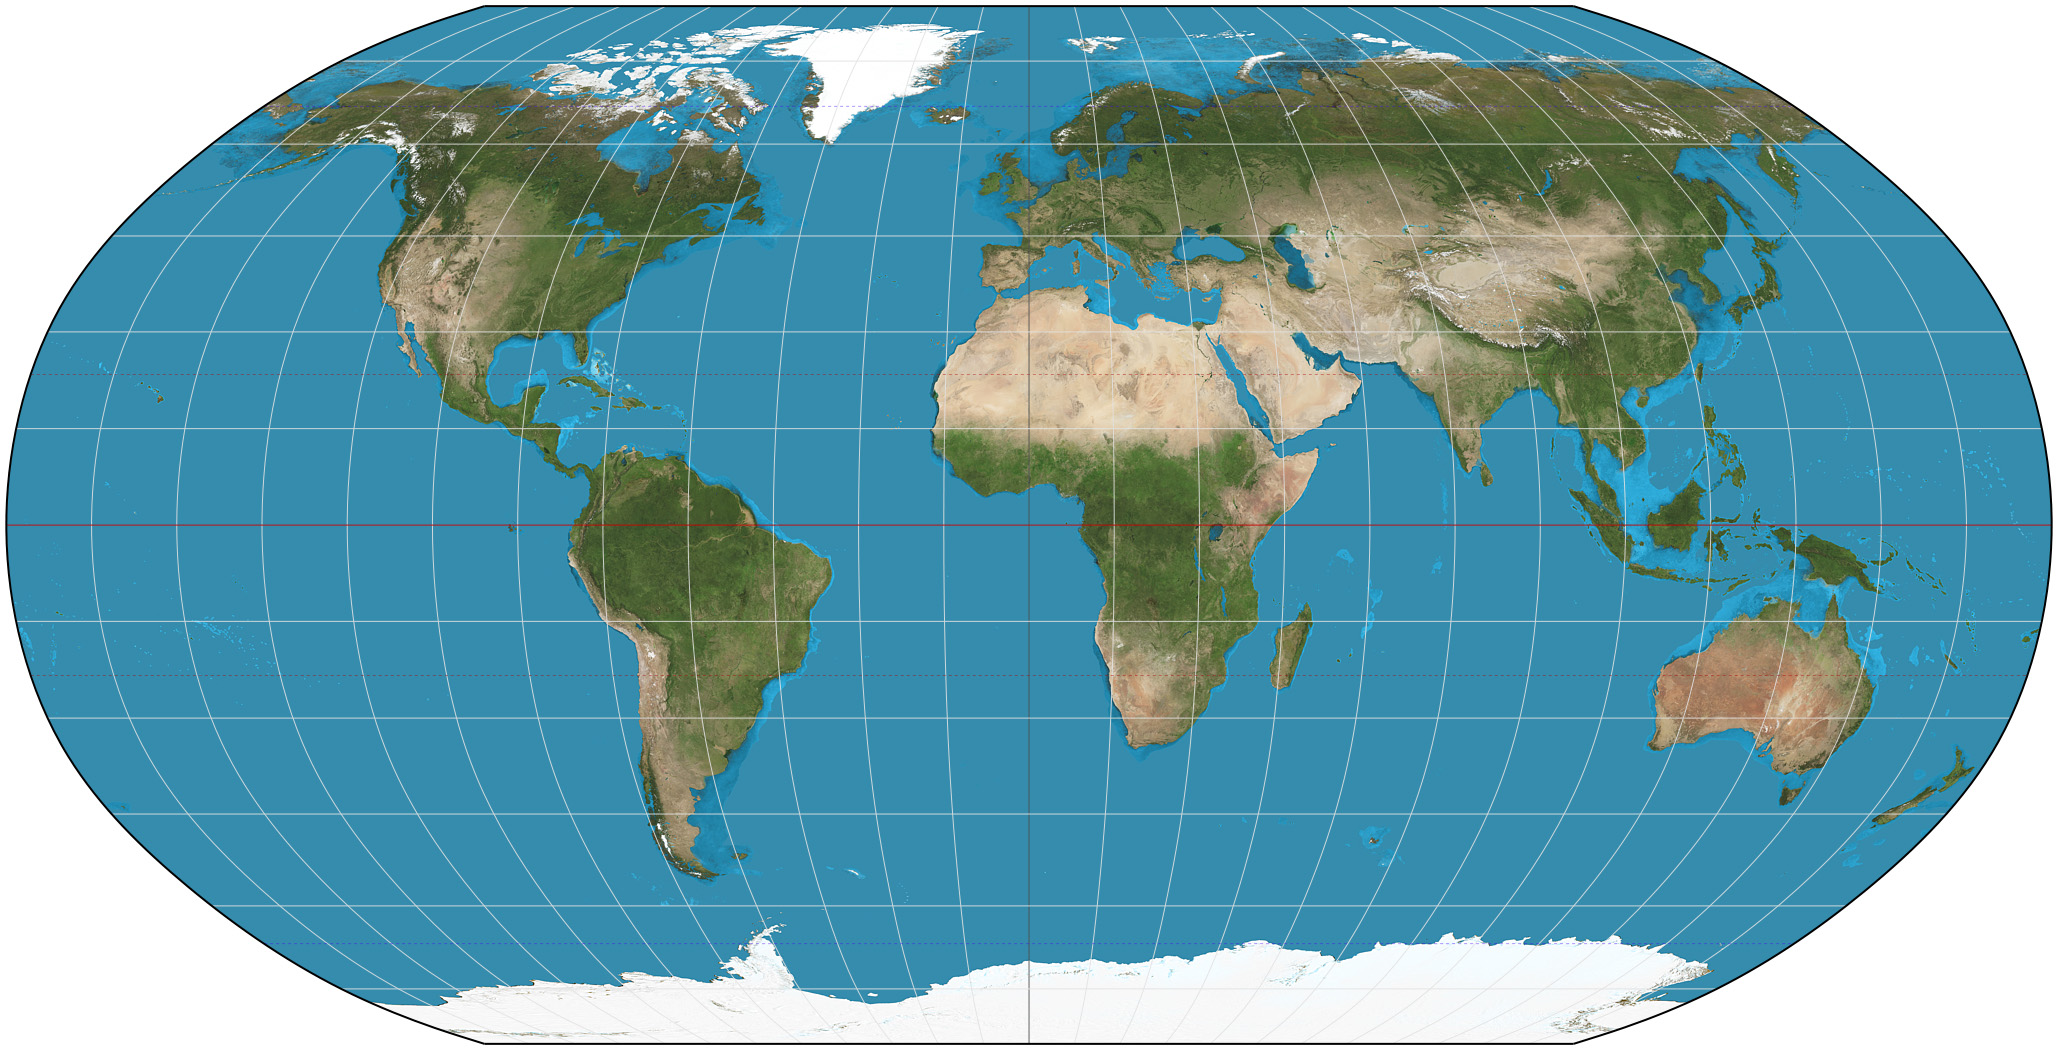
\includegraphics[width=0.55\linewidth, center]{../../website/_assets/milestone1/Robinson_projection.jpg}
\caption{Robinson projection of the world \protect\footnotemark}
\end{figure}
\footnotetext{Daniel R. Strebe, \url{https://en.wikipedia.org/wiki/File:Robinson_projection_SW.jpg}}

\item[3.] Write a function \small\texttt{\detokenize{plot_geo}} \normalsize that creates a plot of the Earth surface type $g_{ij}$ against the mapped coordinates $(x_{ij}, y_{ij})$.
\item[4.] Use these functions in a program and run it to check your results.
\end{enumerate}


\newpage

\section{Bonus}

\begin{enumerate}
\item Implement the Winkel tripel projection, as an alternative to the Robinson projection, given by
\[
\begin{aligned}
	x\left(\theta, \varphi \right) &= \frac{1}{2}\left(\varphi \cos\left(\theta_1\right) + \frac{2\cos(\theta)\sin\left(0.5 \varphi\right)}{\sinc(\alpha)}\right),\\[0.1cm]
	y\left( \theta, \varphi \right) &= \frac{1}{2}\left(\theta + \frac{\sin(\theta)}{\sinc(\alpha)}\right),\\[0.1cm]
	\alpha(\theta, \varphi) &= \arccos\left(\cos(\theta)\cos(0.5 \varphi)\right),
\end{aligned}
\]
where $\theta_1$ is the standard parallel and $\sinc$ is the unnormalized sine function that are
\[
\theta_1 = \arccos\left(\frac{2}{\pi}\right)
\quad
\text{and}
\quad
\sinc(x) = 
\begin{cases}
\frac{\sin(x)}{x} & x \ne 0 \\[0.1cm]
1 & x = 0
\end{cases},
\]
respectively.
\item Write a function to read in other data sets, like ICE-5G\footnote{https://www.atmosp.physics.utoronto.ca/~peltier/data.php}, originally presented and analyzed by Peltier\footnote{Peltier, W.R., Global glacial isostasy and the surface of the ice-age Earth: the ICE-5G (VM2) model and GRACE. Annual Review of Earth and Planetary Sciences, May 2004, Vol 32, 111-149.}. This function should parse this (binary) data which is provided in netCDF format. The data is given on an enriched grid, e.g., with 1$^\circ$ resolution ($360 \times 180$ points) or $10'$ resolution ($2160 \times 1080$ points). So, this read-in routine should also have the option to downsample the data in some way while maintaining an equirectangular grid in lat/lon coordinates.

After readin (and downsampling), write another routine that can categorize the Earth surface types $g_{ij} \in \{1;2;3;5\}$ based on RGB color values for plotting.
The $land=1$, $ice=3$, and $ocean=5$ masking can be done in a straightforward way from the \small\texttt{\detokenize{orog}} \normalsize data is the surface elevation which is positive for land and negative for ocean. Also, the \small\texttt{\detokenize{sftgit}} \normalsize and \small\texttt{\detokenize{sftgif}} \normalsize data provides information about the land ice sheets. Sea ice is trickier to determine and one needs to combine some strategy with CLIMAP to determine the sea ice. This is how the original data from Zhuang et al. created their data.

Note, that the netCDF format may store the latitude and longitude in a different orientation than expected, e.g., South to North rather than North to South. Thus, some reordering of the points is necessary.

%\item Write a function to read in NASA satellite images, e.g., from the Blue Marble Next Generation\footnote{NASA's Goddard Space Flight Center, 2004, \url{https://svs.gsfc.nasa.gov/12564}}, which categorizes the earth surface types $g_{ij} \in \{1;2;3;5\}$ based on RGB color values.
%\item Implement a 3D visualization.
%Plot a map mesh design based on the satellite image using a projection method of your choice.
\end{enumerate}

\newpage

\section{Control Solutions}


\begin{figure}[!htb]

\includegraphics[width=0.99\linewidth]{../../website/_assets/milestone_results/milestone1_geo.png}
\caption{Robinson projection output}
\end{figure}

\end{document}
